\documentclass[serif, english, brazilian, oneside]{uffstex}
\usepackage[utf8]{inputenc}
\usepackage[T1]{fontenc}
\usepackage[
  style=abnt-numeric,
]{biblatex}

\usepackage[useregional=num]{datetime2}
\usepackage{xcolor}
\usepackage{booktabs}
\usepackage{csquotes}
\usepackage{newtxtext}
\usepackage{newtxmath}
\usepackage{cleveref}
\usepackage{siunitx}
\usepackage[pdftex]{hyperref}
\usepackage[
  linesnumbered,
  lined,
  boxed,
  commentsnumbered
]{algorithm2e}

\providecolor{uffsgreen}{RGB}{0, 105, 62}

\addbibresource{refs.bib}

% Comandos de dados
\autor{Cauan Mulinari e Lucas Kauã dos Santos Belini}
\titulo{Trabalho integrador}
\subtitulo{Parte 1: Identificação da empresa e requisitos funcionais}
\curso{Ciência da Computação}
\cidade{Chapecó}
\uf{SC}
% datetime2 não funciona com \today porque ambos formatam a data
\data{\hoje}
\orientador{a}
\coorientador{a}

\begin{document}
\pretextual%

\imprimircapa%

\pdfbookmark{\listfigurename}{lof}
\listoffigures*
\cleardoublepage%

\pdfbookmark{\contentsname}{toc}
% Versão com * não coloca o próprio sumário no sumário
\tableofcontents*
\cleardoublepage%

% Início da parte textual
\textual%

\chapter{Introdução}

Este trabalho tem como objetivo a união das matérias de Engenharia de Software, Banco de Dados e Programação para a produção de um sistema destinado a uma determinada empresa real, que será entrevistada e, a partir da entrevistas, todos os requisitos do sistema serão levantados para que uma solução seja encontrada e produzida.

\chapter{Informações sobre a empresa}

A empresa escolhido pela dupla para a realização do trabalho integrador é a empresa Agro Insumos Ronda Alta LTDA, registrada sob CNPJ número 03.968.063/0001-24, atuando no ramo de insumos agrícolas, comercializando defensivos (herbicidas, fungicidas, inseticidas, acaricidas), implementos agrícolas (plantadeiras da marca vence tudo, peças), sementes (de milho, soja, trigo), adubos e fertilizantes para o solo.

\section{Entrevista com a empresa}

Para a produção dos requisitos da solução, uma entrevista foi realizada com um dos seus colaboradores, Scheila Mulinari, auxiliar administrativa da empresa. Durante a entrevista, diversas perguntas a colaboradora foram realizadas, com o intuito de entender como a empresa trabalha e atua atualmente, além de saber mais sobre o sistema que a empresa utiliza no momento, seus pontos positivos e necessidades que ainda não foram sanadas.

A entrevistada comentou que o sistema utilizado atualmente pela empresa é o AGER, um sistema fornecido pela Wonder Sistemas, que no momento proporciona tudo que a colaboradora necessita. O sistema atual possui um controle de estoque, carteira de clientes e emissão de notas fiscais para o controle financeiro.

A colaboradora entrevistada trabalha com pedidos e vendas utilizando o sistema AGER. Atualmente, quando um cliente realiza uma compra pela empresa, o colaborador é responsável por criar um pedido de venda dentro do sistema, onde o mesmo fica esperando pela retirada do cliente, para que então, ocorra uma baixa no estoque e a nota fiscal seja emitida.

Um dos problemas encontrados atualmente se dá na parte da baixa do estoque, que é realizado apenas na retirada do produto, fazendo com que apenas uma unidade de determinado item consiga ser comprada por diferentes clientes, até que a retirada seja feita.

Uma captura de tela do sistema atual utilizado pela empresa pode ser vista na \autoref{fig:sistema_atual_print}

\newpage

\begin{figure}[!htpb]
    \centering
    \caption{Captura de tela do sistema atual}
    \label{fig:sistema_atual_print}
    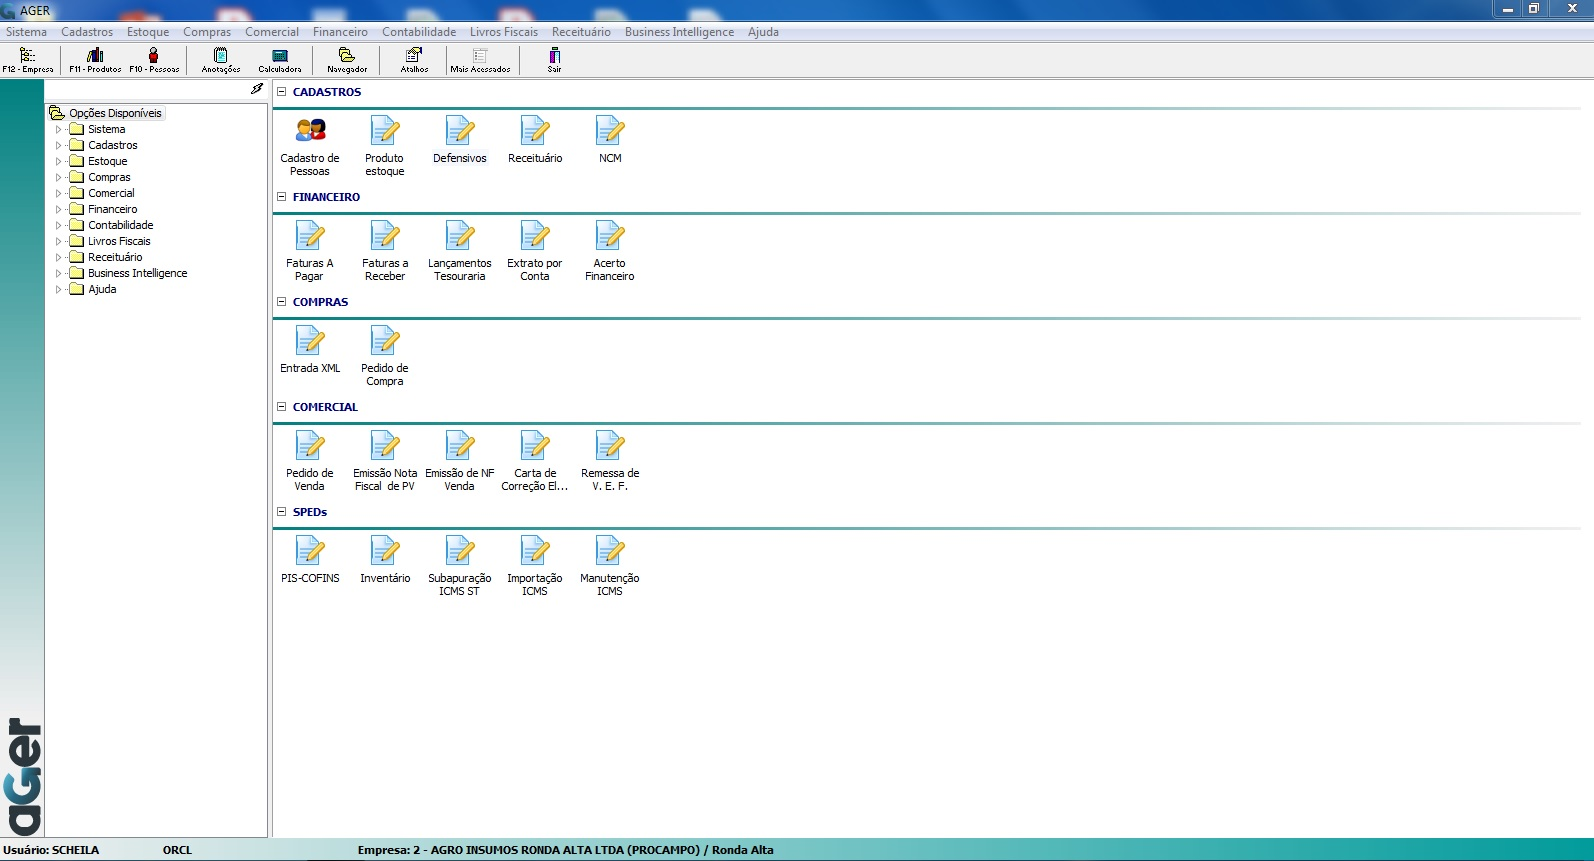
\includegraphics[width=\linewidth]{imagens/sistema_atual.jpeg}
    \legend{Fonte: captura de tela.}
\end{figure}

\section{Expectativas das funcionalidades de um novo sistema}

Durante a entrevista, foi relatado que a empresa possui as seguintes necessidades:

\begin{itemize}
    \item O sistema deverá ser capaz de registrar clientes, guardando o nome, telefone, endereço e CPF dos mesmos;
    \item O sistema deverá ser capaz de registrar produtos, guardando o nome, código de barras e quantidade no estoque;
    \item O sistema deverá ser capaz de registrar pedidos de vendas, que deverá ser atrelado a uma lista de produtos;
    \item O sistema deverá marcar um produto de um pedido como entregue ou, aguardando entrega;
    \item O sistema deverá ser capaz de identificar a falta de um produto no estoque durante a criação do pedido de venda;
    \item O sistema não deverá realizar um pedido de venda de produtos disponíveis no estoque mas, que ainda não foram retirados.
\end{itemize}

\section{Solução encontrada}

A solução encontrada pelo grupo para o problema atual da empresa é: desenvolver um sistema que possua uma carteira de usuários, além de realizar o gerenciamento do estoque da mesma, sendo capaz de solucionar o problema atual dos pedidos de vendas, realizando uma baixa no estoque no momento do pedido.

\chapter{Especificações dos requisitos}



\section{Requisitos funcionais e não funcionais}

Após a entrevista, a dupla foi responsável pelo levantamento e catalogação dos requisitos que o sistema possui, categorizando os mesmos em requisitos funcionais ou requisitos não funcionais.

\subsection{Requisitos funcionais}

De acordo com Fernando Cunha \cite{requisitos-o-que-sao}, os requisitos funcionais são problemas e necessidades resolvidos através do uso de software e, sabendo disso, o grupo propôs uma tabela contendo todos os requisitos funcionais da solução desenvolvida, disponível na \autoref{fig:tabela_req_funcionais}.

\newpage

\begin{figure}[!htpb]
    \centering
    \caption{Tabela de requisitos funcionais da solução encontrada}
    \label{fig:tabela_req_funcionais}
    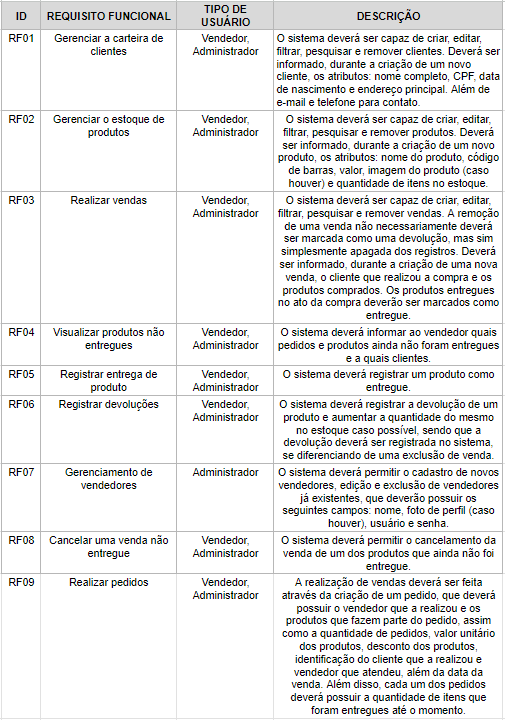
\includegraphics[width=\linewidth]{imagens/tabela_req_funcionais.png}
    \legend{Fonte: autoria própria.}
\end{figure}

\subsection{}{Requisitos não funcionais}

Os requisitos não funcionais, segundo Fernando Cunha \cite{requisitos-o-que-sao}, não descrevem o que o sistema deverá possuir, mas sim como o sistema deverá implementar ou fazer algo.

Para que a construção do sistema fosse possível, o grupo organizou uma tabela com alguns requisitos não funcionais que a aplicação deverá possuir, que pode ser visto na \autoref{fig:req_nao_funcionais}.

\begin{figure}[!htpb]
    \centering
    \caption{Tabela de requisitos não funcionais da solução encontrada}
    \label{fig:req_nao_funcionais}
    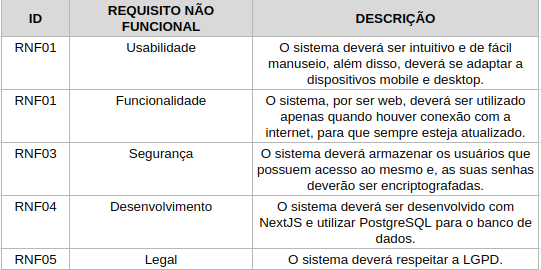
\includegraphics[width=\linewidth]{imagens/req_nao_funcionais.png}
    \legend{Fonte: autoria própria.}
\end{figure}

\section{Diagrama de caso de uso}

De acordo com um artigo públicado no website LucidChart \cite{diagrama-de-caso-de-uso}, um diagrama de caso de uso é utilizado para representar as interações entre os diferentes tipos de usuários, chamados de atores, com o sistema.

\subsection{Atores do diagrama de caso de uso}

\begin{figure}[!htpb]
    \centering
    \caption{Tabela dos atores do diagrama de caso de uso}
    \label{fig:atores_caso_uso}
    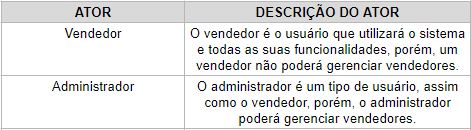
\includegraphics[width=0.7\linewidth]{imagens/atores_diagrama_caso_uso.png}
    \legend{Fonte: autoria própria.}
\end{figure}


\printbibliography[heading=abnt]

\end{document}